%
% teil1.tex -- praktische Anwendung
%
\section{Praktische Anwendung}
\kopfrechts{Praktische Anwendung}%

\subsection{Einleitung}

Im folgenden Abschnitt wird praktische Anwendung von Reynolds-Averaging gezeigt.
\index{Anwendung}%
Anhand von einer Beispielsimulation werden verschiedene Turbulenzmodelle verglichen, und es wird auf deren Stärken und Schwächen eingegangen.
Es ist dabei jedoch esentiell zu verstehen, dass auch mit optimalem Trubulenzmodell eine Simulation einer turbulenten Strömung immer noch nur eine Näherung ist,
und keinesfalls blind darauf vertraut werden sollte.

\subsection{Simulationsdomäne}
\label{subsubsec:domain-desc}

Um dem Leser oder der Leserin ein möglichst praxisrelevantes Verständnis der Problematik zu vermitteln, werden
im nachfolgenden Teil Beispiele von CFD-Simulationen gezeigt.
Dabei wird die in Grafik~\ref{fig:SimDomain} gezeigte Geometrie verwendet.
Die Geometrie ist immer vollständig mit Wasser (\SI{25}{\degreeCelsius}) gefüllt,
auf der linken Seite ist ein Einlass mit Einlassgeschwindigkeit \SI{10}{\meter\per\second} definiert und
auf der rechten Seite ein Auslass auf Umgebungsdruck.
Das Mesh\footnote{``Mesh'' bezeichnet die Unterteilung des zu simulierenden Volumens in einzelne Zellen,
in denen die Navier-Stokes-Gleichung gelöst werden.} ist so gewählt, dass es in der Tiefe nur ein Element hat,
bzw. so dass die Simulation einer zweidimensionalen Simulation entspricht.

\begin{figure}
    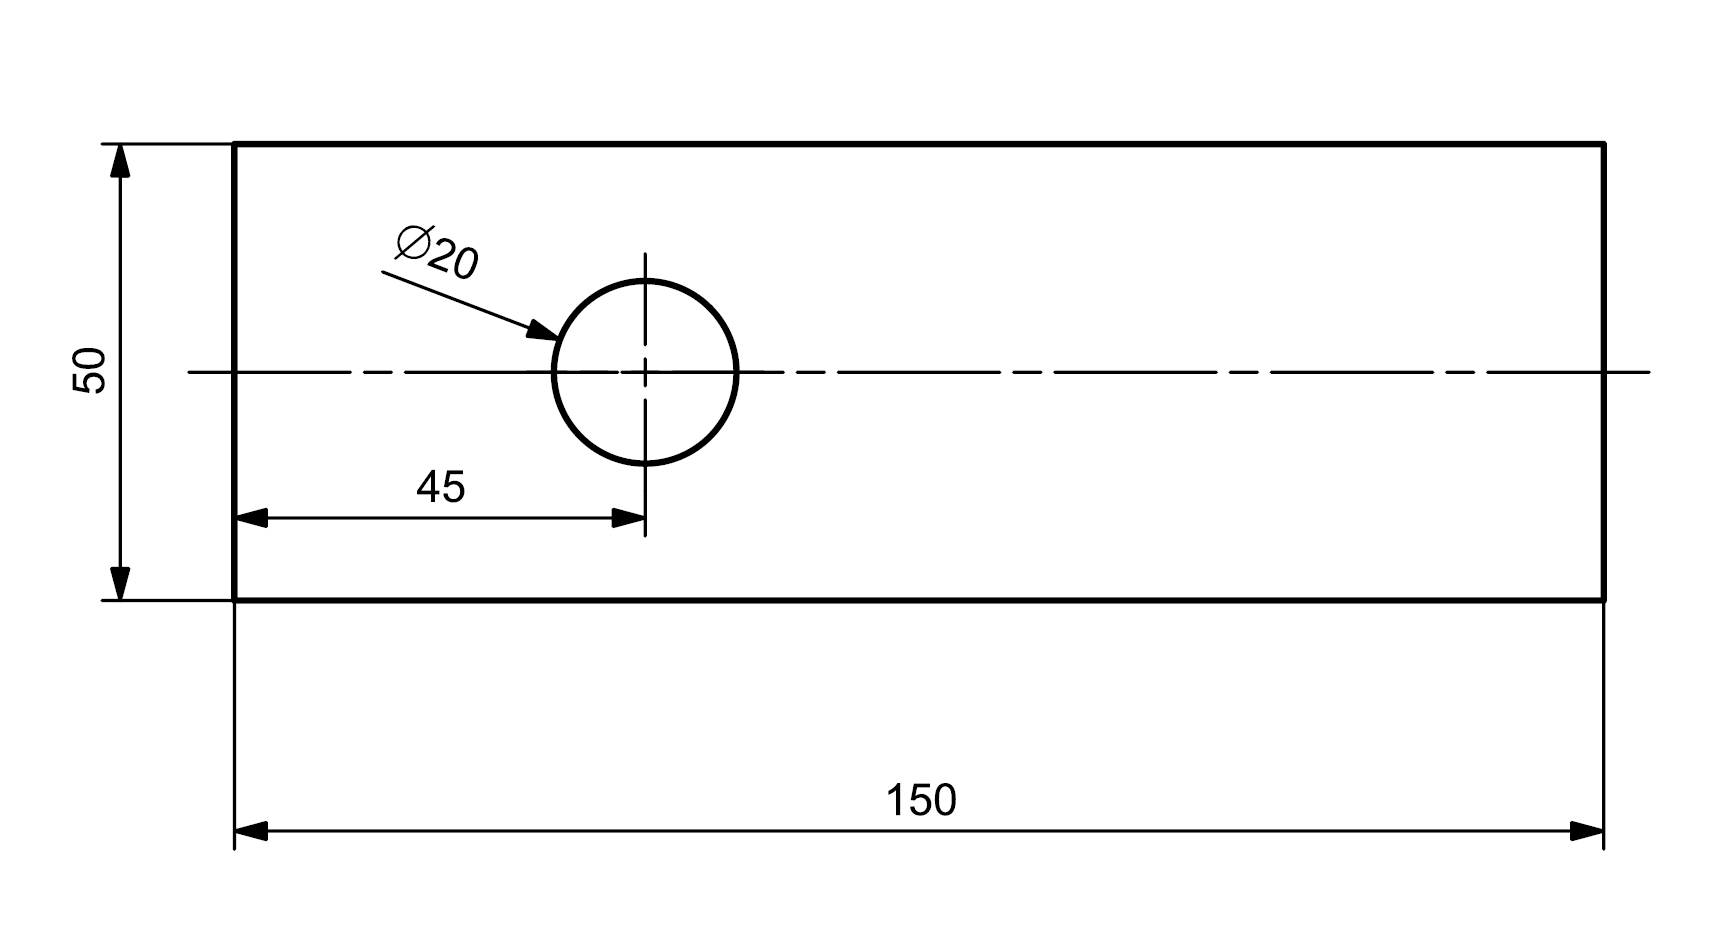
\includegraphics[width=\textwidth]{papers/reynolds/images/domain.png}
    \caption{Simulationsgeometrie}
    \label{fig:SimDomain}
\end{figure}

\subsection{Verschiedene Turbulenzmodelle}

Viele prominente Turbulenzmodelle bestehen aus zwei Skalarfeldern.
Es gibt jedoch auch zusammengesetzte Modelle, die aus mehreren Modellen bestehen.
Dabei gibt es zusammengesetzte Modelle, die für verschiedene Bereiche der Simulation verschiedene Modelle benützen,
um die jeweiligen Begebenheiten besser zu repräsentieren,
sowie zusammengesetzte Modelle, die zeitliche und räumliche Mittelung in einem Modell vereinen.
Je komplizierter ein Modell, desto höher ist auch der Rechenaufwand.

Das wohl meistverbreitete Turbulenzmodell ist das k-$\epsilon$-Modell, das mit zwei Feldern auskommt. Das k-Feld für die
\index{k-epsilon-Modell@k-$\epsilon$-Modell}%
turbulente kinetische Energie, und das $\epsilon$-Feld für die Eddy-Viskosität, welche eine aufgrund der Turbulenzen errechnete
\index{Eddy-Viskositat@Eddy-Viskosität}%
hypothetische Viskosität darstellt.
Folgend eine nicht vollständige Liste von Turbulenzmodellen für RANS:

\begin{itemize}
    \item k-$\epsilon$
    \item k-$\omega$
\index{k-omega-Modell@k-$\omega$-Modell}%
    \item Shear Stress Transport (SST) (Kombination aus k-$\epsilon$ und k-$\omega$)
\index{SST}%
\index{Shear Stress Transport}%
    \item Quadratisch/Kubisch k-$\epsilon$
    \item RANS-LES kombiniertes Modell ($\ge 4$ Felder)
\index{RANS-LES}%
\end{itemize}

Jedes dieser Turbulenzmodelle hat seine Eigenheiten und spezifischen Einsatzbereiche.
So ist das k-$\epsilon$ Modell zum Beispiel nicht geeignet für schwach turbulente Strömungen,
wo es die Effekte der Verwirbellung tendenziell überschätzt (siehe Abbildung~\ref{fig:k-e}).
Das k-$\omega$-Modell ist in diesem Bereichen besser geeignet, wie man in Abbildung~\ref{fig:k-w}
erkennen kann. Das SST-Modell kombiniert die beiden Modelle, so dass im Wandbereich,
wo die meisten Turbulenzen auftreten, k-$\epsilon$ verwendet wird und um im mittleren Bereich,
wo die Turbulenzen schwächer ausgeprägt sind, k-$\omega$ verwendet wird.
Aufgrund dieser Charakteristik ist das SST-Modell auch eines der realistischsten Modelle,
benötigt jedoch drei Felder (k, $\epsilon$ und $\omega$), was den Rechenaufwand erhöht.
In den Bildern~\ref{fig:ohne}, \ref{fig:k-e}, \ref{fig:k-w} und \ref{fig:SST}
wird ein Vergleich zwischen den verschiedenen Modellen sowie eine Simulation ohne
Reynolds-Averaging gezeigt.

\begin{figure}
  \centering
  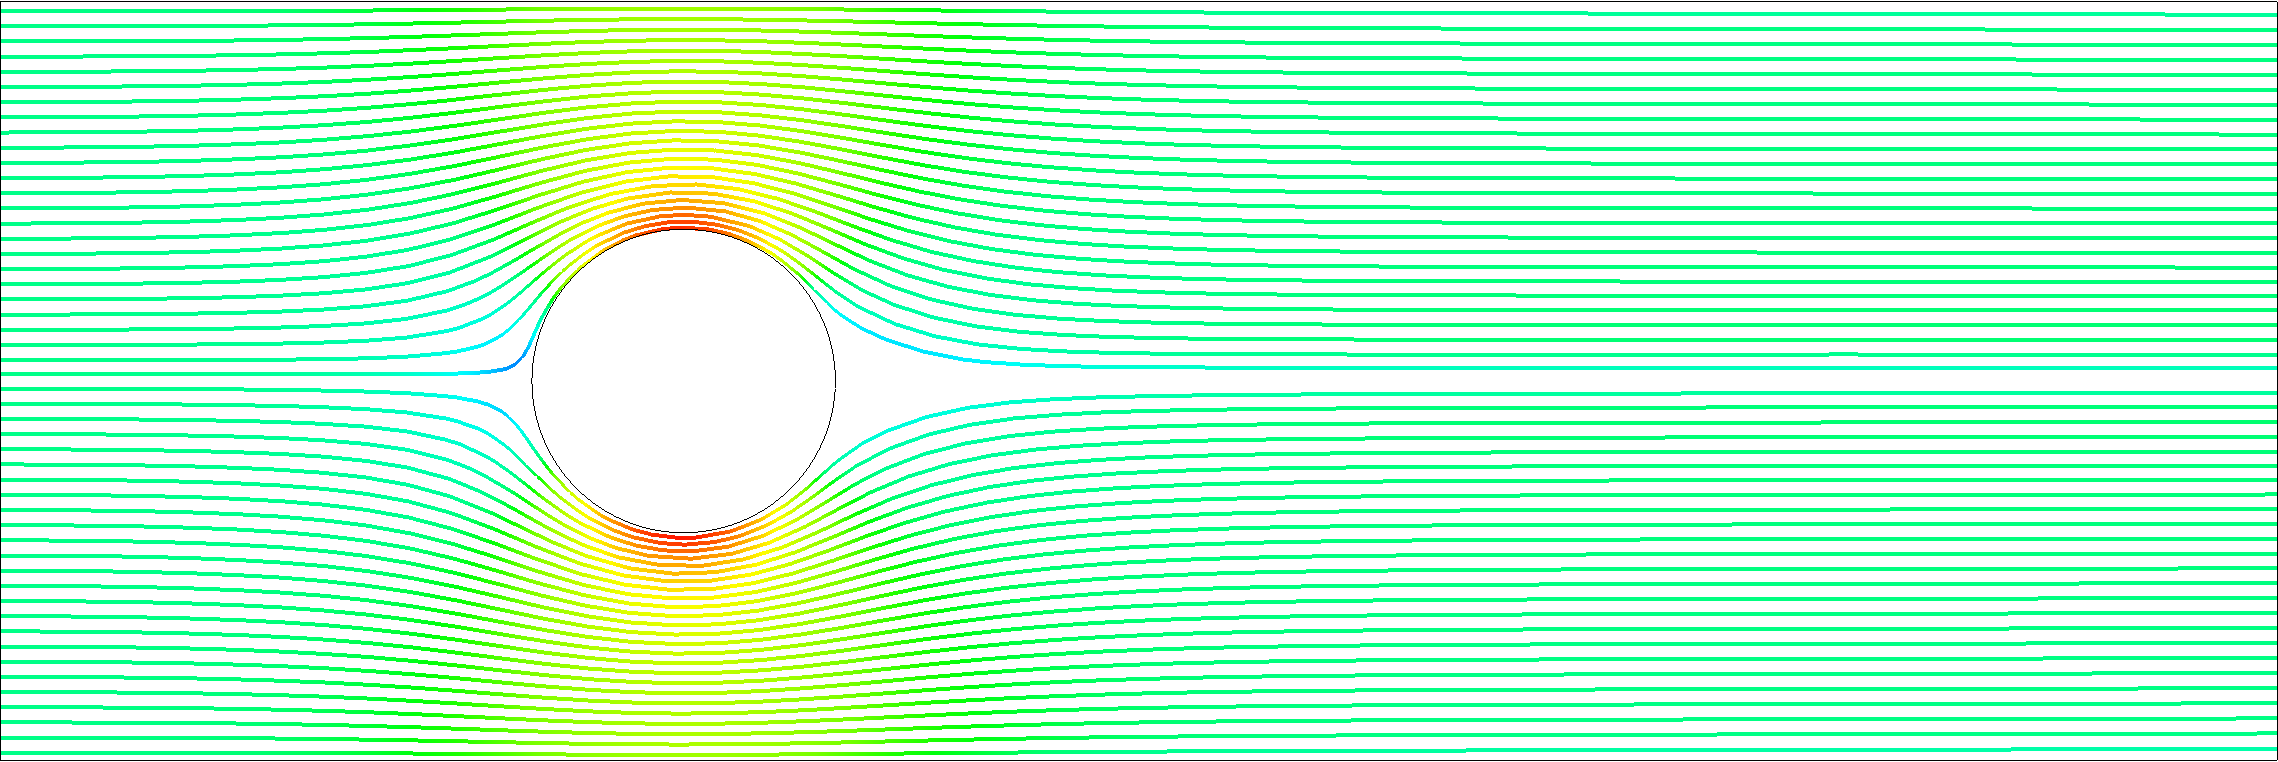
\includegraphics[width=0.99\textwidth]{papers/reynolds/croppedimages/dns.png}
  \vspace*{-6pt}
  \caption{Ohne Reynolds-Averaging}
  \label{fig:ohne}
  \vspace*{6pt}
  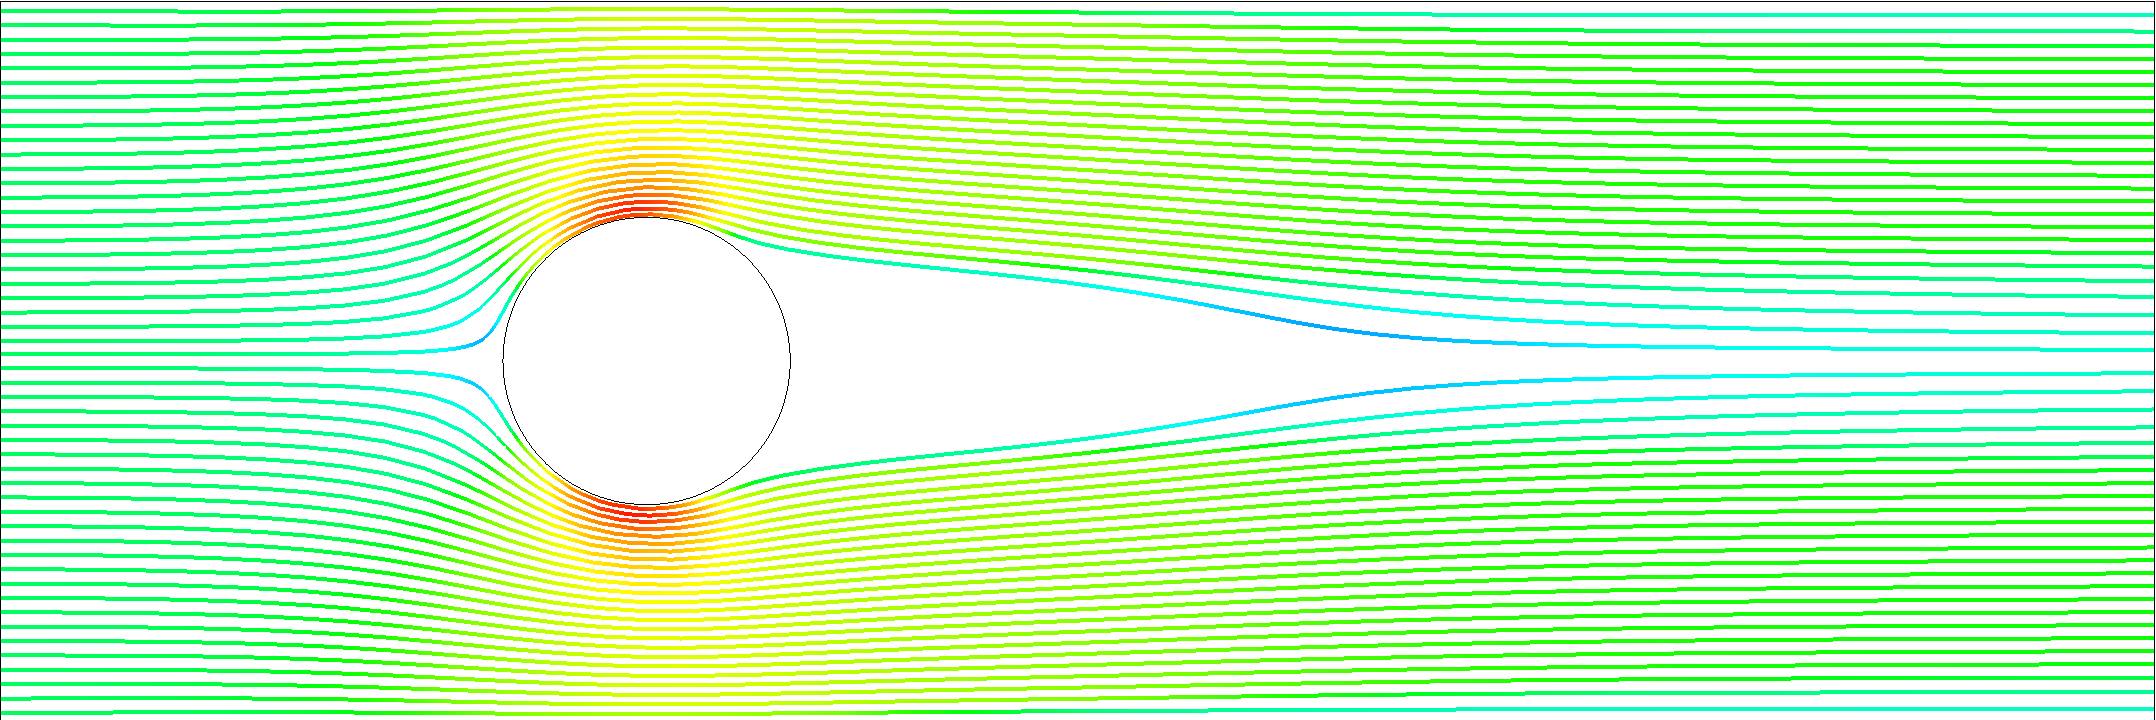
\includegraphics[width=0.99\textwidth]{papers/reynolds/croppedimages/k-e.png}
  \vspace*{-6pt}
  \caption{Mit k-$\epsilon$ Turbulenzmodell}
  \label{fig:k-e}
  \vspace*{6pt}
  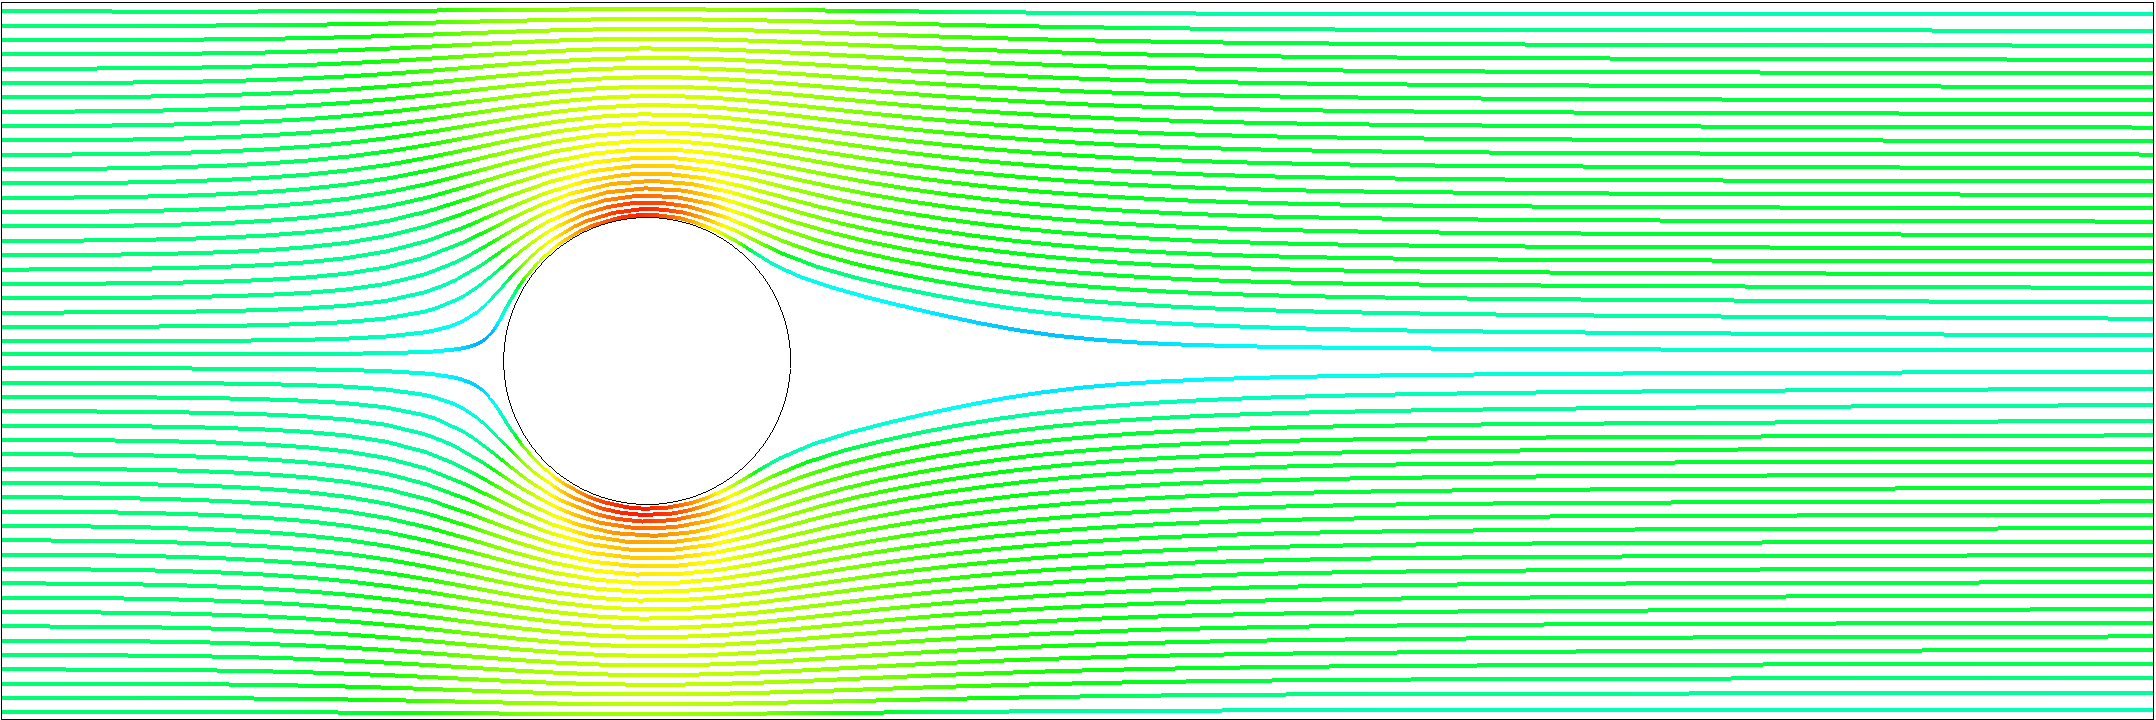
\includegraphics[width=0.99\textwidth]{papers/reynolds/croppedimages/k-w.png}
  \vspace*{-6pt}
  \caption{Mit k-$\omega$ Turbulenzmodell}
  \label{fig:k-w}
  \vspace*{6pt}
  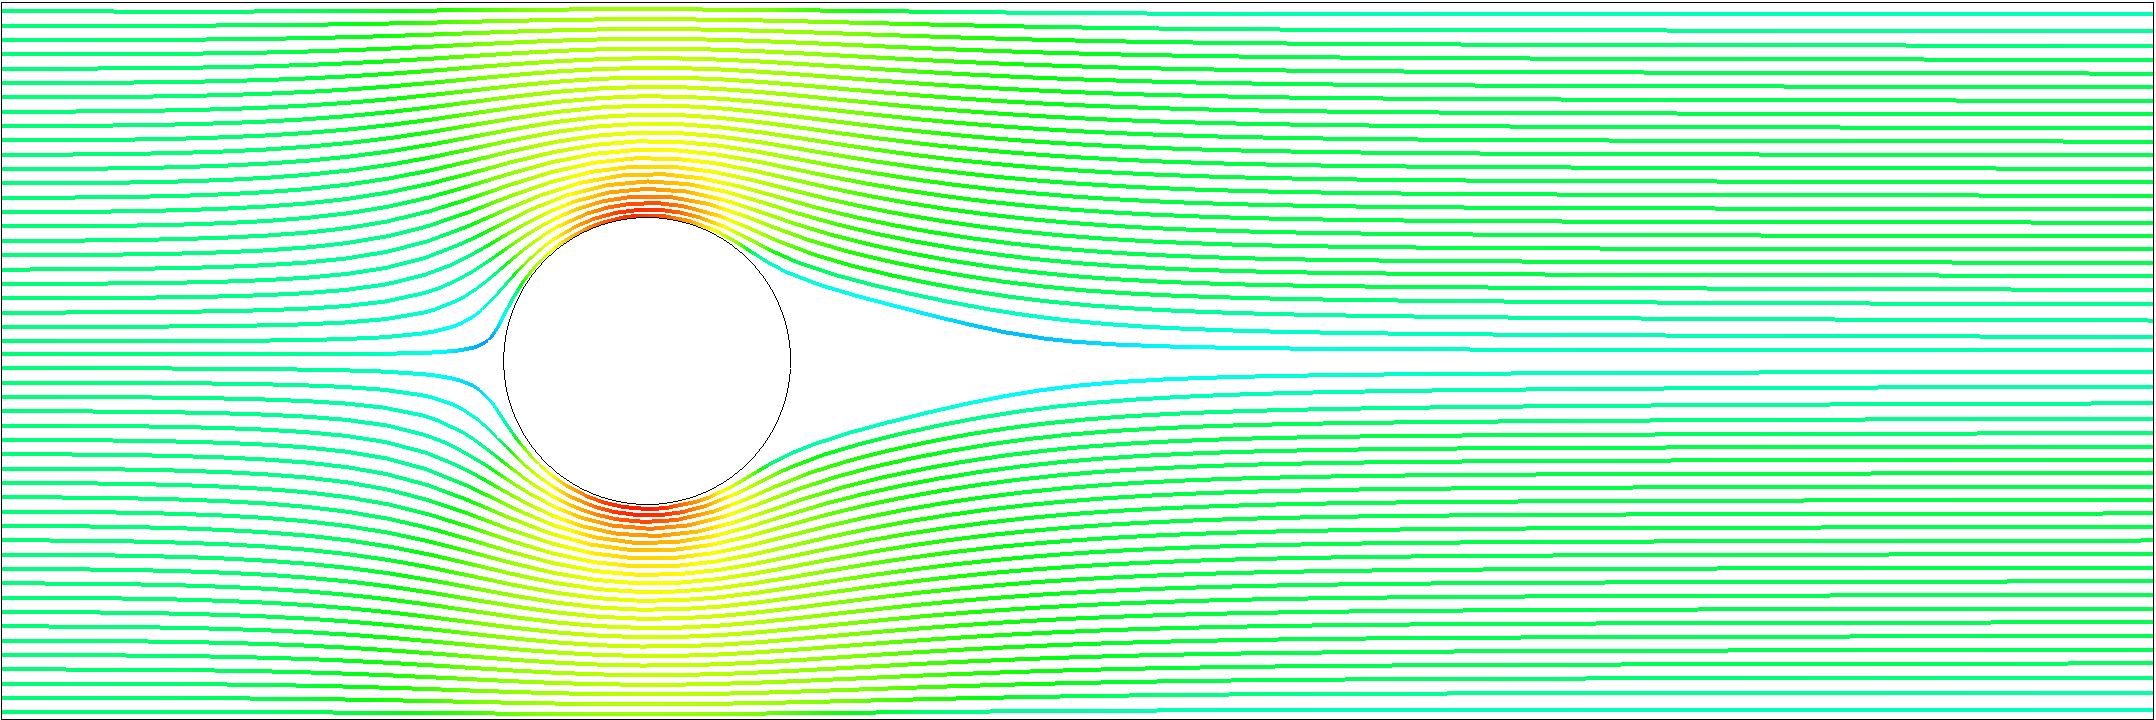
\includegraphics[width=0.99\textwidth]{papers/reynolds/croppedimages/sst.png}
  \vspace*{-6pt}
  \caption{Mit SST Turbulenzmodell}
  \label{fig:SST}
\end{figure}

Die Verwendung des passenden Turbullenzmodells erfordert viel Erfahrung sowie ein gutes 
praktisches Verständnis der simulierten Strömung. Auch muss an dieser Stelle nochmals erwähnt werden,
dass durch die Verwendung von Turbulenzmodellen Simulationen von turbulenten Strömungen bestenfalls eine Näherungen sind.
Darum werden CFD-Simulationen vorwiegend für Optimierungsprobleme eingesetzt, da mehrere Simulationen in Relation zu einander
oft relativ genau sind (vorausgesetzt die Grenze zwischen laminar und turbulent befindet sich nicht im simulierten Bereich).
Wenn man also zum Beispiel in der in Abschnitt \ref{subsubsec:domain-desc} beschriebenen Simulation den Kreis durch ein
eiförmige Geometrie ersetzen würde, könnte man in den Simulationsergebnissen eine klare Veränderung feststellen.
Diese Veränderung würde in den meisten Fällen auch ungefähr der Veränderung in der Realität entsprechen,
die Ergebnisse der einzelnen Simulationen stimmen jedoch meist nicht wirklich mit den realen Begebenheiten überein.


